%
% 02_konstruktion.tex -- SchrittweiseKonstruktion des Beweises
%
% (c) 2026 Dominik Castelberg, Ostschweizer Fachhochschule
%
% !TEX root = ../../buch.tex
% !TEX encoding = UTF-8
%
\section{Konstruktion des Beweises
\label{jordan:section:konstruktion}}
\kopfrechts{Naive Ansätze für den Beweis}

\subsection{Der naive Ansatz Form-spezifischer Beweise}

Wie bereits erwähnt, ist der Satz von Jordan für spezielle Kurvenformen wie Kreise oder Ellipsen trivial zu beweisen.
So wäre der Beweis für eine Kreisform $\gamma(t) = (r \cos(2\pi t), r \sin(2\pi t))$ mit $t \in [0,1]$ und $r > 0$ einfach zu führen, da die Kurve die Ebene in ein inneres Gebiet (den Kreis) und ein äußeres Gebiet (die unendliche Fläche außerhalb des Kreises) teilt.

\begin{proof}[Beweis des Jordan'schen Satzes für Kreise]
    Sei $\gamma(t) = (r \cos(2\pi t), r \sin(2\pi t))$ eine geschlossene, einfache Kurve in der Ebene $\mathbb{R}^2$. 
    Das innere Gebiet $I$ ist definiert als die Menge aller Punkte $(x,y)$, die die Ungleichung $x^2 + y^2 < r^2$ erfüllen. 
    Das äußere Gebiet $A$ ist definiert als die Menge aller Punkte $(x,y)$, die die Ungleichung $x^2 + y^2 > r^2$ erfüllen. 
    Die Kurve $\gamma$ selbst bildet die gemeinsame Grenze dieser beiden Gebiete, da sie die Gleichung $x^2 + y^2 = r^2$ erfüllt.    
    Daher hält der Satz von Jordan für Kreise.
\end{proof}

\begin{figure}
    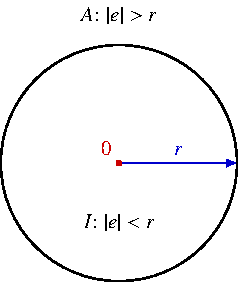
\includegraphics[width=0.8\textwidth]{papers/jordan/images/strategie_kreis.pdf}
    \caption{Aufteilung der Ebene $E$ durch eine Kreisform in ein inneres Gebiet $I$ und ein äußeres Gebiet $A$.}
\end{figure}

Doch dieser Beweis ist stark auf die spezielle Form der Kurve angewiesen und lässt sich nicht auf beliebige geschlossene, einfache Kurven verallgemeinern. 
Da es potentiell unendlich viele verschiedene Formen von geschlossenen, einfachen Kurven gibt, ist es unmöglich, für jede Form einen eigenen Beweis zu führen. 
Dies macht den Ansatz form-spezifischer Beweise unpraktikabel und ineffizient.

\subsection{Beweis für konvexe Polygone\label{jordan:section:konvexe_polygone}}

Konvexe Polygone sind eine weniger restriktive Form von geschlossenen, einfachen Kurven. 
Der Beweis des Jordan'schen Satzes für konvexe Polygone kann aus der Definition der konvexen Hülle als Schnittmenge aller Halbebenen, die alle Eckpunkte des Polygons enthalten, abgeleitet werden.

\begin{definition}[Halbebene]
    Eine Halbebene in der Ebene $\mathbb{R}^2$ ist die Menge aller Punkte, die auf einer Seite einer Geraden liegen. 
    Eine Gerade teilt die Ebene in zwei Halbebenen, wobei jeder Punkt in der Ebene entweder in einer der beiden Halbebenen oder auf der Geraden selbst liegt.
\end{definition}

\begin{definition}[Konvexe Hülle]
    Die konvexe Hülle einer Menge von Punkten $S$ in der Ebene $\mathbb{R}^2$ ist die kleinste konvexe Menge, die alle Punkte in $S$ enthält.
    Die Schnittmenge aller Halbebenen, die alle Punkte in $S$ enthalten, bildet die konvexe Hülle von $S$.
\end{definition}

\begin{figure}
    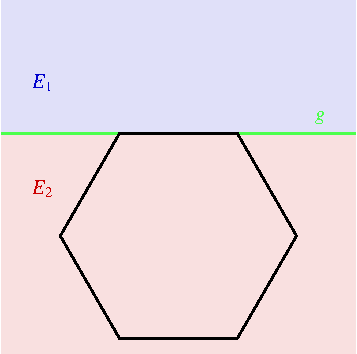
\includegraphics[width=0.8\textwidth]{papers/jordan/images/strategie_konvexe_polygone.pdf}
    \caption{Aufteilung der Ebene $E$ durch eine erweiterte Hexagonseite $g$ in zwei Halbebenen $E_1$ und $E_2$.}
\end{figure}


\begin{proof}[Beweis des Jordan'schen Satzes für konvexe Polygone]
    Sei $\gamma$ ein konvexes Polygon in der Ebene $\mathbb{R}^2$. 
    Das innere Gebiet $G_{inner}$ ist die konvexe Hülle der Eckpunkte des Polygons, während das äußere Gebiet $G_{outer}$ die Menge aller Punkte außerhalb dieser Hülle ist. 
    Die Kurve $\gamma$ selbst bildet die gemeinsame Grenze dieser beiden Gebiete, da sie die Eckpunkte des Polygons verbindet. 
    Daher hält der Satz von Jordan für konvexe Polygone.
\end{proof}

Geschlossene, einfache Kurven können jedoch auch nicht-konvexe Formen annehmen, was den Beweis für konvexe Polygone erneut unzureichend macht, um den Satz von Jordan im Generellen zu beweisen.

\subsection{Beweis für einfache Polygone\label{jordan:section:einfache_polygone}}

Einfache Polygone verwerfen die Einschränkng der Konvexität und erlauben es, dass die Kurve in sich selbst zurückkehrt, solange sie sich nicht schneidet. 
Die Eigenschaft der Konvexität war jedoch in der vorherigen Beweisführung entscheidend, da sie die Definition der konvexen Hülle und die Trennung der Ebene in zwei Gebiete erleichtert hat. 

Wir benötigen daher einen neuen Ansatz, um die bisherigen, durch die Eigenschaften der Konstruktion der behandelten Körper gegebenen, Definitionen für "Innen" und "Aussen" neu zu formulieren. Ein wertvolles Werkzeug ist hierbei die Strahlenparität.

\begin{definition}[Strahlenparität]
    Sei $P$ ein einfaches Polygon und $p \in \mathbb{R}^2 \setminus \partial P$.
    Für jeden strahl $L$ mit Anfangspunkt $p$, der keine Ecke von $P$ trifft und nicht entlang einer Kante von $P$ verläuft, sei $N(p,L)$ die Anzahl Schnittpunkte von $L$ mit $\partial P$. 
    Dann gilt:
    \begin{itemize}
        \item $N(p,L)$ ist endlich.
        \item Die Parität von $N(p,L)$ hängt nicht von $L$ ab, sondern nur von $p$.
    \end{itemize}
\end{definition}

Diese Definition erlaubt es, die Punkte in der Ebene in zwei Mengen zu unterteilen: diejenigen, die eine gerade Anzahl von Schnittpunkten mit dem Polygon haben (die äussere Menge), und diejenigen, die eine ungerade Anzahl von Schnittpunkten haben (die innere Menge).

\begin{definition}[Innen- und Außengebiet]
    Sei $P$ ein einfaches Polygon und $p \in \mathbb{R}^2 \setminus \partial P$. 
    Dann gilt:
    \begin{itemize}
        \item $p$ liegt im inneren Gebiet $I$ von $P$, wenn $N(p,L)$ ungerade ist.
        \item $p$ liegt im äußeren Gebiet $A$ von $P$, wenn $N(p,L)$ gerade ist.
    \end{itemize}
\end{definition}

Um den Satz von Jordan rigoros zu beweisen, müssen wir jedoch noch folgende Punkte zeigen:

\begin{itemize}
    \item $I$ und $A$ sind beide offen und nicht leer.
    \item $I$ und $A$ sind wegzusammenhängend.
    \item $I$ ist beschränkt, während $A$ unbeschränkt ist.
    \item $\partial P$ ist die gemeinsame Grenze von $I$ und $A$.
\end{itemize}

\begin{lemma}[Offenheit von $I$ und $A$]
    Die Parität $N(p,L)$ ändert sich nicht, wenn $p$ innerhalb einer kleinen Umgebung verschoben wird, solange $p$ nicht auf $\partial P$ liegt. 
    Daher sind $I$ und $A$ offen.
\end{lemma}

\begin{lemma}[Nicht-Leerheit von $I$]
    Per Definition kann $I$ nicht leer sein, da Polygone mindestens drei Eckpunkte besitzen müssen, die ein inneres Gebiet definieren. 
    Daher ist $I$ nicht leer.
\end{lemma}

\begin{lemma}[Nicht-Leerheit von $A$]
    Die Absenz von $A$ ist unmöglich, da die Ebene $\mathbb{R}^2$ unbeschränkt ist und es daher immer Punkte gibt, die außerhalb des Polygons liegen.
    Daher ist $A$ nicht leer.
\end{lemma}

Die Etablierung der Wegzusammenhängigkeit von $I$ und $A$ verlangt ein topologisch substantielleres Argument: Die Wegzusammenhängendheitseigenschaften von triangulierten Polygonen. 

\begin{definition}[Triangulierung eines einfachen Polygons]
    Eine Triangulierung eines einfachen Polygons $P$ ist eine Zerlegung von $P$ in nicht überlappende Dreiecke, deren Ecken jeweils Ecken von $P$ sind und die sich paarweise nur in Kanten oder Ecken schneiden.
\end{definition}

\begin{lemma}[Triangulierungssatz für einfache Polygone]
    Jedes einfache Polygon $P$ mit $n \geq 3$ Ecken besitzt eine Triangulierung.
\end{lemma}

%TODO Citation
Dieser Triangulierungssatz wurde 1975 von G. H. Meister präzise bewiesen. Der Beweis basiert auf folgendem Lemma:

\begin{lemma}[Existenz einer Diagonale]
    Jedes einfache Polygon $P$ mit $n \geq 4$ Ecken besitzt eine Diagonale, d.h. eine Linie, die zwei nicht benachbarte Ecken von $P$ verbindet und vollständig innerhalb von $P$ liegt.
\end{lemma}

Die Existenz einer in einem Polygon mit mehr als drei Ecken liegenden Diagonale impliziert, dass das Polygon in zwei kleinere Polygone zerlegt werden kann.

\begin{figure}
    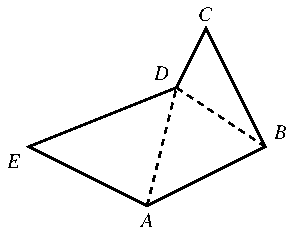
\includegraphics[width=0.8\textwidth]{papers/jordan/images/triangulierung.pdf}
    \caption{Triangulierung eines einfachen Polygons in nicht überlappende Dreiecke.}
\end{figure}

\begin{lemma}[Wegzusammenhängendheit von $I$]
    Sei $P$ ein einfaches Polygon und $I$ das innere Gebiet von $P$. 
    Der Triangulierungssatz für einfache Polygone garantiert, dass jedes $P$ mit $n \geq 3$ Ecken in nicht überlappende Dreiecke zerlegt werden kann.
    Da Dreiecke als konvexe Polygone wegzusammenhängend sind, können wir einen Weg zwischen zwei Punkten in $I$ konstruieren, indem wir die Dreiecke durchqueren, die das Polygon bilden.
    Daher ist $I$ wegzusammenhängend.
\end{lemma}

\begin{lemma}[Wegzusammenhängendheit von $A$]
    Sei $P$ ein einfaches Polygon, $I$ das innere Gebiet von $P$, $A$ das äußere Gebiet von $P$, und $K$ das innere Gebiet eines Kreises, welche $P$ umschliesst, ohne es zu berühren, und $A$ das äußere Gebiet von $P$. 
    Da $A$ unbeschränkt ist, können wir einen Weg von einem Punkt $k \in K \setminus P \cup I$ zu einem Punkt $a \in A$ konstruieren, der keine Punkte von $P$ enthält. 
    Daher ist $A$ wegzusammenhängend.
\end{lemma}

\begin{lemma}[Beschränktheit von $I$]
    Sei $P$ ein einfaches Polygon und $I$ das innere Gebiet von $P$. 
    Da $P$ eine endliche Anzahl von Ecken hat, ist die konvexe Hülle von $P$ beschränkt. 
    Daher ist auch $I$ beschränkt.
\end{lemma}

\begin{lemma}[Unbeschränktheit von $A$]
    Sei $P$ ein einfaches Polygon und $A$ das äußere Gebiet von $P$. 
    Da die Ebene $\mathbb{R}^2$ unbeschränkt ist, gibt es immer Punkte, die außerhalb der konvexen Hülle von $P$ liegen. 
    Daher ist $A$ unbeschränkt.
\end{lemma}


\begin{proof}[Gemeinsame Grenze von $I$ und $A$]
    Sei $P$ ein einfaches Polygon, $I$ das innere Gebiet von $P$, und $A$ das äußere Gebiet von $P$.
    Die Kurve $\partial P$ bildet eine gemeinsame Grenze von $I$ und $A$, da jeder Punkt auf $\partial P$ sowohl adjazent zu Punkten in $I$ als auch adjazent zu Punkten in $A$ liegt.
    Sie ist die einzige gemeinsame Grenze, da $I$ per Definition durch $P$ begrenzt ist.
\end{proof}

In Kombination führen diese Lemmas und Definitionen zu einem vollständigen Beweis des Jordan'schen Satzes für einfache Polygone.

%TODO: Ausformulierung Beweis

\subsection{Beweis für Reel-analytische Kurven}

%TODO Einführung

\subsubsection{Fortführung des Strahlenparitäts-Arguments}

%TODO Tubenumgebung

%TODO Verallgemeinerung der Strahlenparität auf analytische Kurven

%TODO Warum unnötig kompliziert

\subsubsection{Pivotpunkt: Nutzung der Umlaufzahl}

%TODO Tangentenwindungszahl

%TODO Hopfscher Umlaufsatz

In \ref{buch:integration:cauchy:subsetion:umlaufzahl} wurde die Umlaufzahl eines Weges um einen Punkt eingeführt.

\subsection{Beweis für Stückweise C\textsuperscript{1}-Kurven}

%TODO Gauss-Bonnet Modifikation

\subsection{Beweis für Stetige Kurven}

%TODO Approximierung durch einfache Polygone (lokale Approximation)

%TODO Überleitung zur Alexander-Dualität